\documentclass[./4_GeneralApproach.tex]{subfiles}
\graphicspath{{\subfix{../../Images}}}

\begin{document}
Fig. \ref{fig:contract_based_architecture} summarises the contract-based specification of the general system.

\begin{figure}[htp]
    \centering
    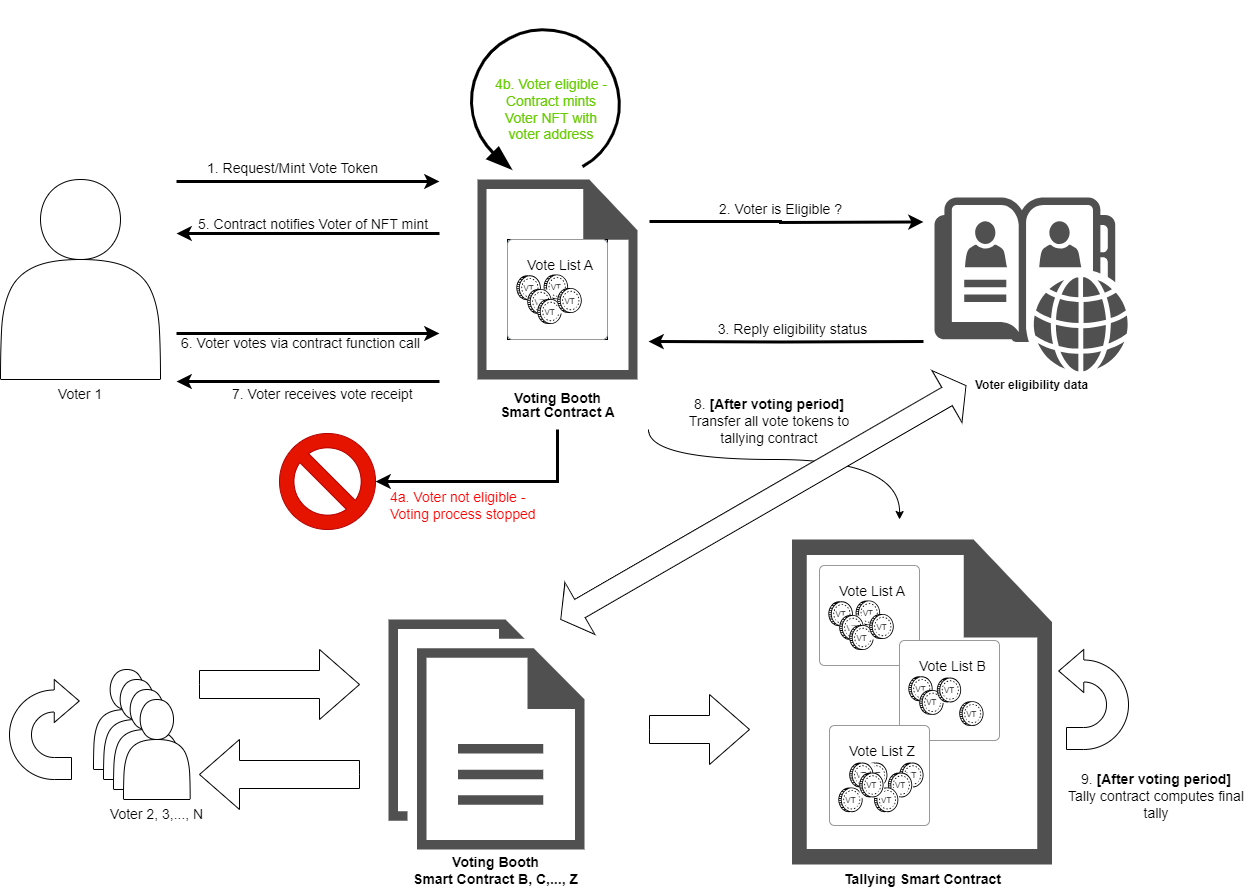
\includegraphics[width=0.7\textwidth]{../Images/02_contract_based_solution.png}
    \caption{Contract-based version of the e-voting system proposed.}
    \label{fig:contract_based_architecture}
\end{figure}

The crucial aspect to take into account with this version is how contract-based blockchains store smart contract-related data. All data related to a smart contract, from token ownership records to token metadata (in the case of NFT-generating smart contracts), is stored "into" the contract, i.e., in a block array referenced from the block where the contract was deployed. The details of how this storage is processed are beyond the scope of this document, but this fact exposes a security issue that requires addressing since contract-based blockchains are quite common, and we intend to implement this version of the solution in Ethereum, perhaps the best example of such a blockchain.
\par
Encrypting the data using the public key from an asymmetrical encryption key pair is the most obvious solution and one we intend to explore to mitigate this issue. Regardless of the simplicity of the approach, there are several options on how to employ this encryption layer that require careful consideration first. We identified four potential approaches to address vote data privacy:

\begin{itemize}
    \item{\textbf{Each voting booth smart contract uses a different public key from an asymmetric encryption pair to encrypt any sensible information before setting it as the NFT's metadata.} Smart contract code is transparent once it is published on the blockchain, so it is not possible for the contract to store the private key from that pair without invalidating the encryption itself.
          \par
          To maintain a level of decoupling, voting booth smart contracts can only encrypt data while keeping decryption functionalities limited to the tallying contract. This is not a limitation of the technology but a security strategy. The transparency argument also applies to the tally contract, which means that we cannot store any private encryption keys in it without invalidating the encryption scheme. As we have established in Section \ref{general_approach}, our solutions assume the existence of a trusted third party, which can be used to store the private pairs of the encryption keys used, under reasonable safety. This encryption problem can be solved by implementing the decryption function in the tally contract only, but in such a way that it requires the private encryption keys to be provided as inputs to the function as well as the data to be decrypted. Fig. \ref{fig:multiple_encryption_key_scheme} exemplifies the process described thus far.
          \par
          The system is more secure if each voting booth smart contract uses a different encryption key, but this security comes at the cost of increased system complexity. Decrypting the data requires multiple inputs, and a single erroneous byte in the transmission of one of the private keys can invalidate the whole election.}

          \begin{figure}[htp]
              \centering
              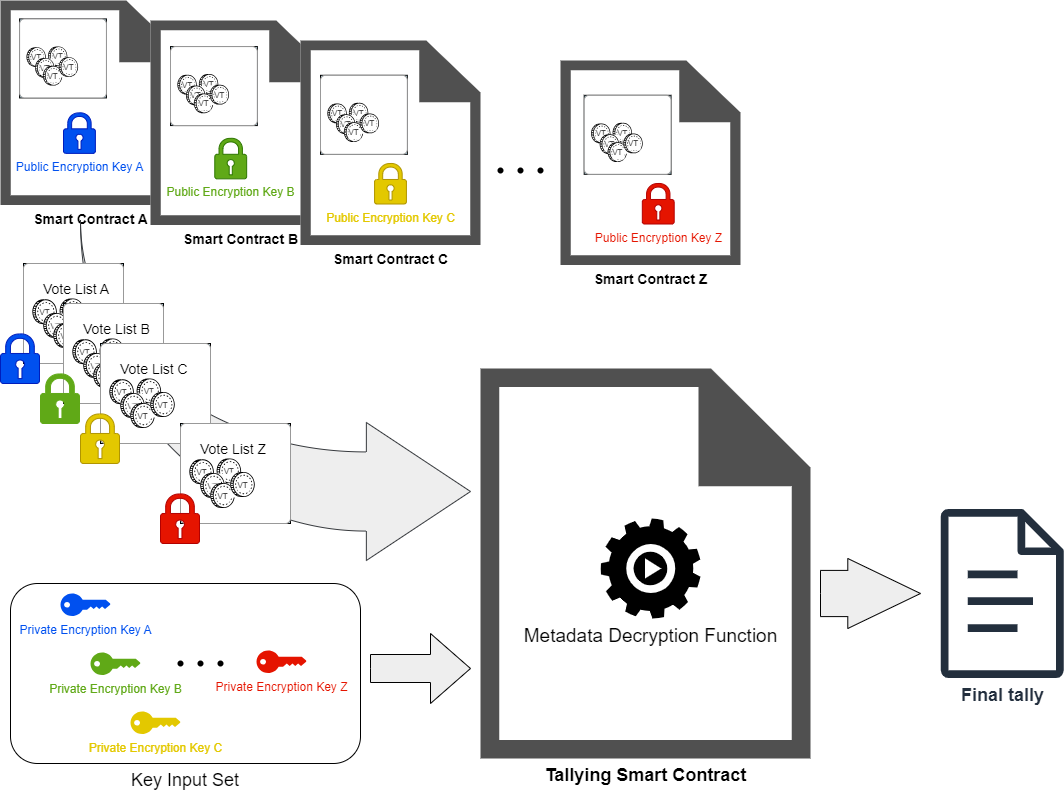
\includegraphics[width=0.7\textwidth]{../Images/ContractBasedSolution_encryption1.png}
              \caption{Metadata encryption scheme using multiple encryption key pairs.}
              \label{fig:multiple_encryption_key_scheme}
          \end{figure}

    \item{\textbf{All voting booth smart contracts use the same public key from an asymmetrical encryption pair to protect NFT metadata.} This approach is functionally similar to the previous one but logistically simpler because all NFT metadata is encrypted with the same key.
          \par
          In this case, only one encryption key pair gets generated, with the public key freely distributed and used over the whole system and the private key safely guarded by a trusted third party. As with the previous case, voting booth smart contracts can only encrypt data, with the decrypting responsibilities falling solely on the tallying contract and the correct input of the private encryption key from the trusted third party.
          \par
          In this alternative, the trade-off benefits system complexity (or lack thereof) to the detriment of security. It is logistically simpler to keep a single key secure than multiple ones. Fig. \ref{fig:single_encryption_key_scheme} illustrates this approach.}

          \begin{figure}[htp]
              \centering
              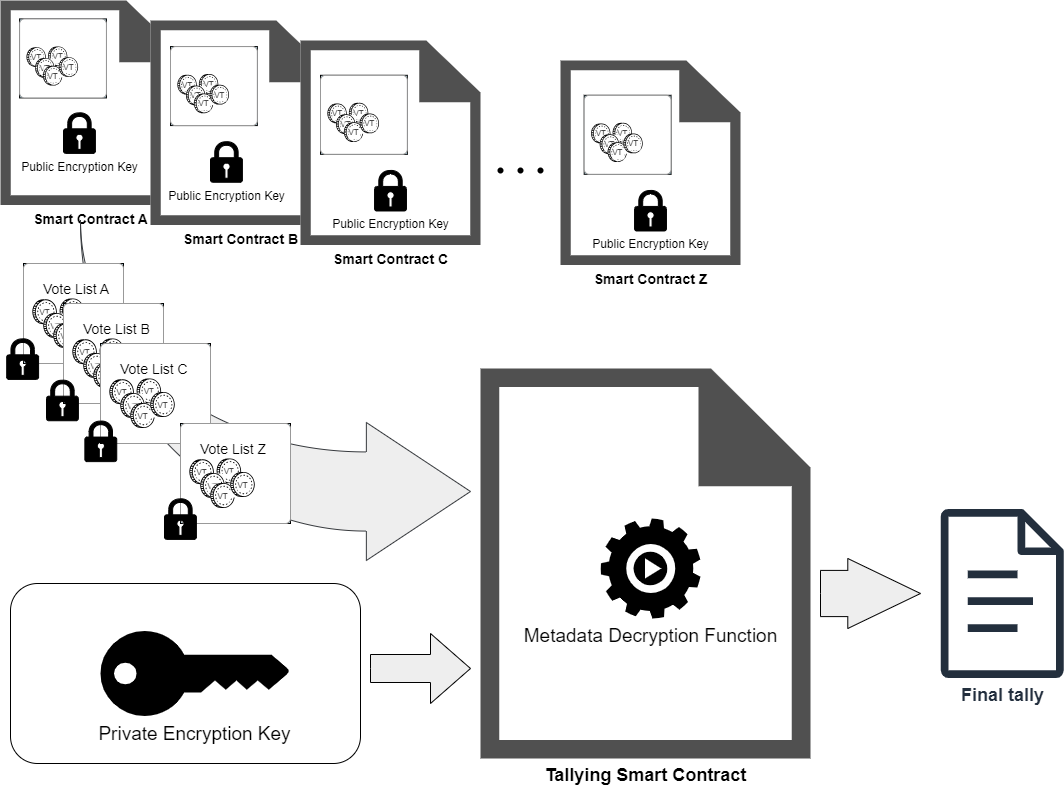
\includegraphics[width=0.7\textwidth]{../Images/ContractBasedSolution_encryption2.png}
              \caption{Metadata encryption scheme using a single encryption key pair.}
              \label{fig:single_encryption_key_scheme}
          \end{figure}

    \item{\textbf{Use a threshold cryptosystem and homomorphic properties} to keep vote data encrypted throughout the whole process. If a threshold cryptosystem is used to encrypt the vote data, we can use homomorphic operations directly on the encrypted data to calculate a (still encrypted) final tally, the only element requiring decryption in this scenario \cite{Benaloh1986b} \cite{Rjaskova2002}.}

    \item{\textbf{Use Adi Shamir's Secret Sharing scheme \cite{Shamir1979}} to split a private key $ D $ from an asymmetrical encryption key pair into $ n $ pieces. Shamir's secret sharing scheme requires that only $ k $ of these pieces be able to reconstruct $ D $. This scheme also requires the use of a \textit{(k, n)} threshold cryptosystem, where $ n = 2k - 1 $. With such a scheme, an adversary needs to obtain at least $ k $ pieces to be able to subvert the system while being able to use a single encryption key for all. As long as an adversary is unable to obtain as many as $ k - 1 $ pieces, reconstructing $ D $ is still computationally infeasible. This scheme effectively combines the advantages of the first two discussed with a minimal increment in solution complexity.}
\end{itemize}
\end{document}